% Chapter Template

\chapter{Results and Discussions} % Main chapter title

\label{Chapter 4} % Change X to a consecutive number; for referencing this chapter elsewhere, use \ref{ChapterX}

\lhead{Chapter 4. \emph{Results and Discussions}} % Change X to a consecutive number; this is for the header on each page - perhaps a shortened title

%----------------------------------------------------------------------------------------
%	SECTION 1
%----------------------------------------------------------------------------------------

\section{Github API Server}
As per our objectives defined, we were able to deliver all the required functionalities within the maximum possible latency limit defined. Some of the various functionalities were:
\begin{description}

\item[$\bullet$] List admins, given the repository name and the organization name.

\item[$\bullet$] Create a repository given the organization.

\item[$\bullet$] Change the visibility of a repository, given the organization and the repository.

\item[$\bullet$] Update the permissions of an external collaborator, given the collaborator name, permission status, repository name and the organization name.

\item[$\bullet$] Remove a collaborator from a repository, given the collaborator name, the repository name and the organization name.

\item[$\bullet$] Delete a repository, given the repository, given the organization and the repository name.

\item[$\bullet$] List all repositories, given the organization.

\item[$\bullet$] List all the members, given the organization.

\item[$\bullet$] List all outside collaborators, given the repository and the organization.

\item[$\bullet$] Add external collaborator to a repository, given the collaborator name, repository name and the organization name.

\item[$\bullet$] Get the Github login id, given the NTID of a user.

\item[$\bullet$] List all organizations of the enterprise.

\end{description}

These are the list of utility functions.
\begin{description}

\item[$\bullet$] getPAT() - Fetch the Personal access token from Azure key vault.

\item[$\bullet$] getSAML() - Fetch the list of mapping from Github id to NTID.

\item[$\bullet$] exeGraphql() - Execute a graphql query using HTTP Post request to Github API and retrieve the response.

\item[$\bullet$] Execute-HTTP-POST() - Make a HTTP Post request by adding headers and required JSON body and send it to Github API.

\item[$\bullet$] Execute-HTTP-PUT() - Make a HTTP Put request by adding headers and required JSON body and send it to Github API.

\item[$\bullet$] Execute-HTTP-Patch() - Make a HTTP Patch request by adding headers and required JSON body and send it to Github API.

\item[$\bullet$] Execute-HTTP-DELETE() - Make a HTTP Delete request by adding headers and required JSON body and send it to Github API.

\end{description}
Here are some of the output screenshots:

\begin{figure}[H]
\centering
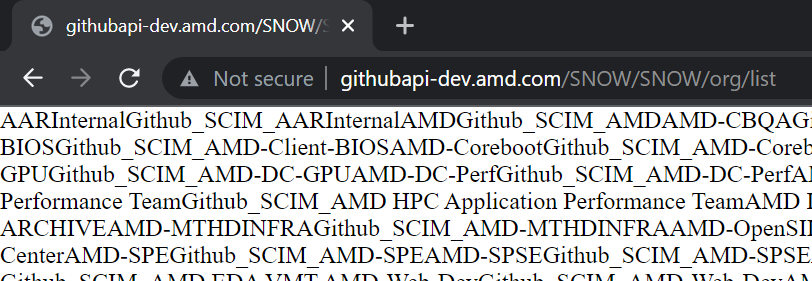
\includegraphics[width = .8\textwidth]{Images/SNOWORGLIST}
\caption{Output - List of Organizations}
\label{List of organizations}
\end{figure}

\begin{figure}[H]
\centering
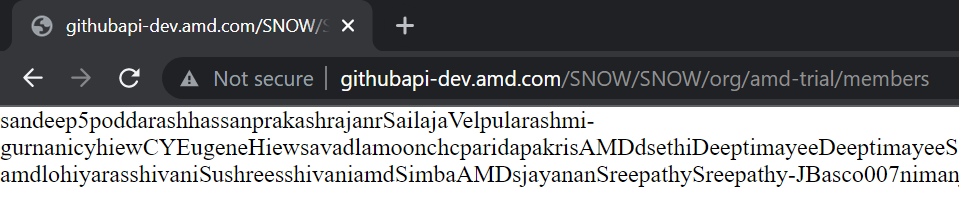
\includegraphics[width = .8\textwidth]{Images/LISTMEMBERS}
\caption{Output - List of members in an organization}
\label{List of members in an organization}
\end{figure}

\begin{figure}[H]
\centering
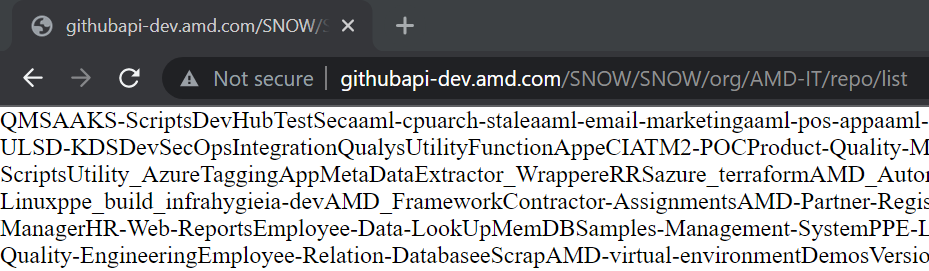
\includegraphics[width = .8\textwidth]{Images/LISTREPOS}
\caption{Output - List of repositories of an organization}
\label{List of repositories in an organization}
\end{figure}


\section{Github Runner}
As per our objectives defined for the Github Runner, we were able to stand up the Github runner with the capabilities as requested by various organizations. It is able to successfully listen to jobs and communicate back the result.

Here are some of the output screenshots:

\begin{figure}[H]
\centering
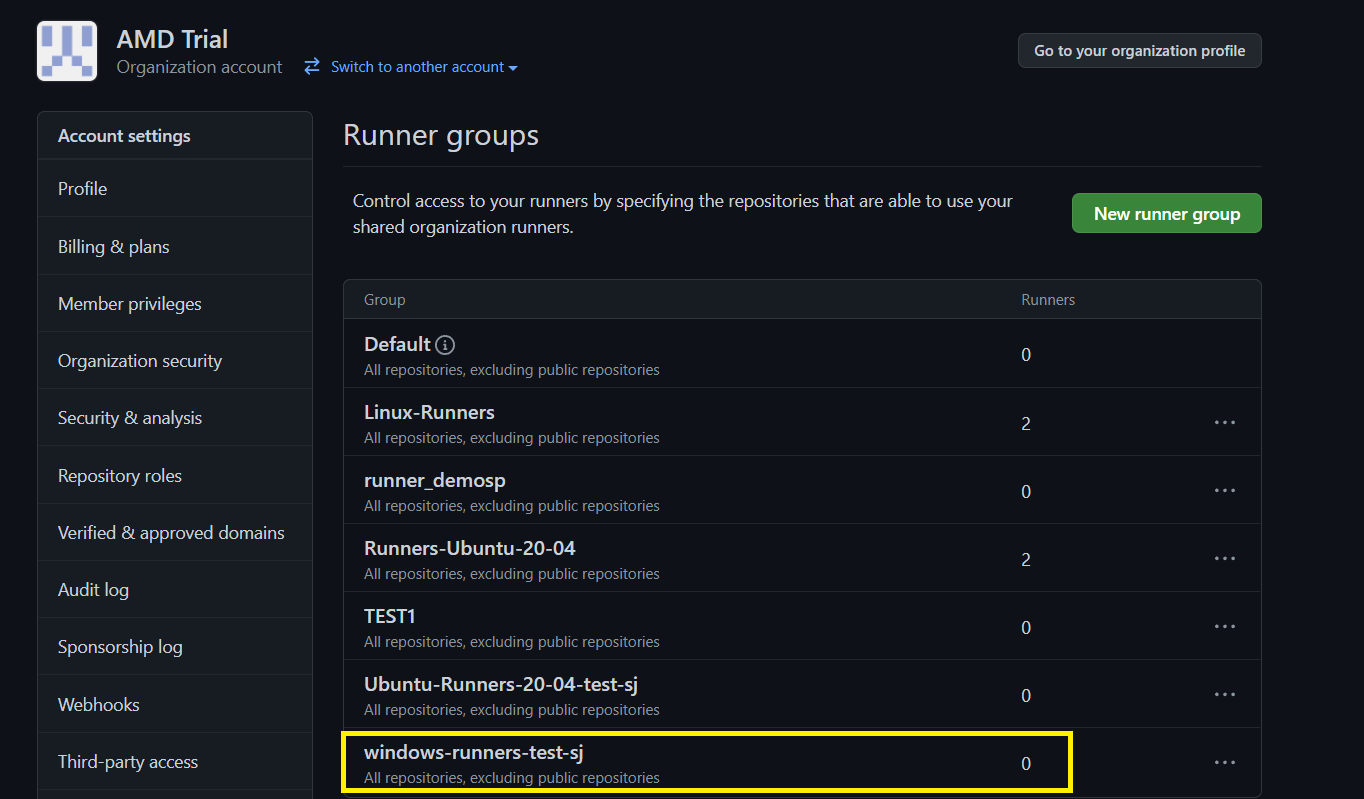
\includegraphics[width = 1\linewidth]{Images/RUNNER1}
\caption{Output - Count of runners in the runner group "windows-runners-test-sj" before adding the runner}
\label{Count of runners in the runner group "windows-runners-test-sj" before adding the runner}
\end{figure}

\begin{figure}[H]
\centering
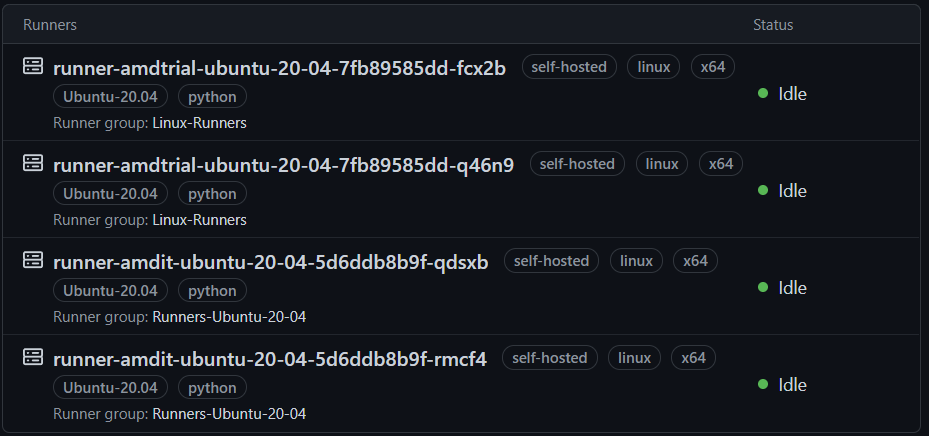
\includegraphics[width = 1\linewidth]{Images/RUNNER4}
\caption{Output - List of runners before adding the runner}
\label{List of runners before adding the runner}
\end{figure}

\begin{figure}[H]
\centering
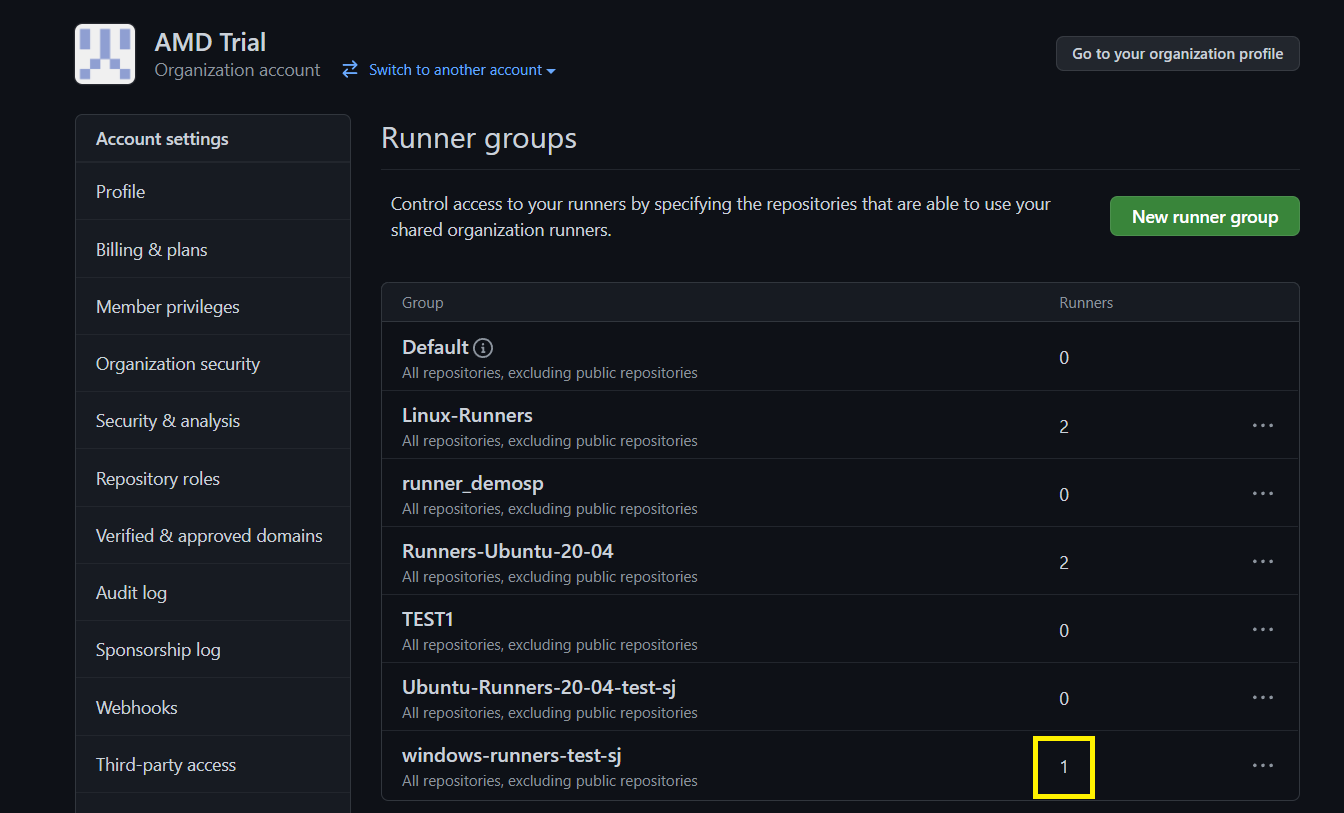
\includegraphics[width = 1\linewidth]{Images/RUNNER3}
\caption{Output - Count of runners in the runner group "windows-runners-test-sj" after adding the runner}
\label{Count of runners in the runner group "windows-runners-test-sj" after adding the runner}
\end{figure}

\begin{figure}[H]
\centering
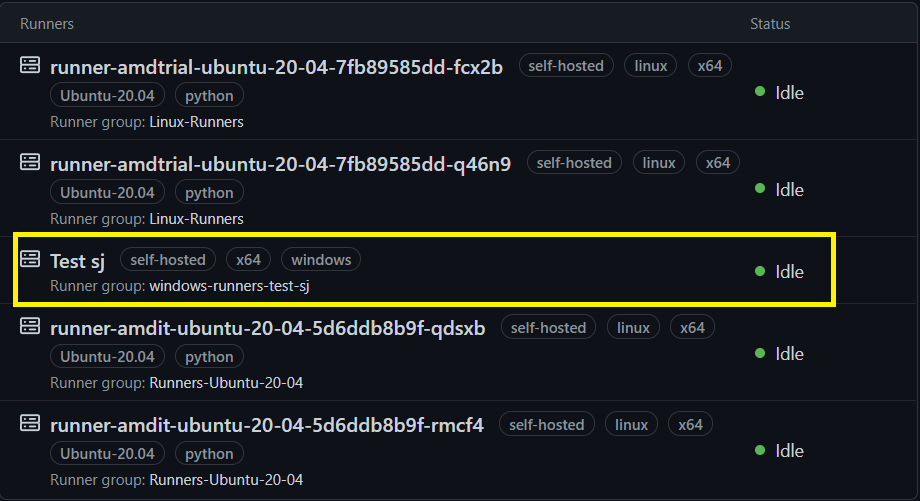
\includegraphics[width = 1\linewidth]{Images/RUNNER2}
\caption{Output - List of runners after adding the runner}
\label{List of runners after adding the runner}
\end{figure}

You can see that the runner "Test sj", inside the runner group "windows-runners-test-sj" is in the idle state and is actively looking for the workloads to be given.